\documentclass{article}
\usepackage{amsmath}
\usepackage{amssymb}
\usepackage{amsfonts}
\usepackage[T1]{fontenc}
\usepackage{bm}
\usepackage{array}
\usepackage{graphicx}
\usepackage[utf8]{inputenc}
\usepackage{tikz}
\usetikzlibrary{shapes.geometric, arrows}
\tikzstyle{rec} = [rectangle,  minimum width=2cm, minimum height=1cm, text centered, draw=black]
\tikzstyle{arrow} = [thick,->,>=stealth]

\begin{document}

\begin{figure}[htpb]
\begin{center}
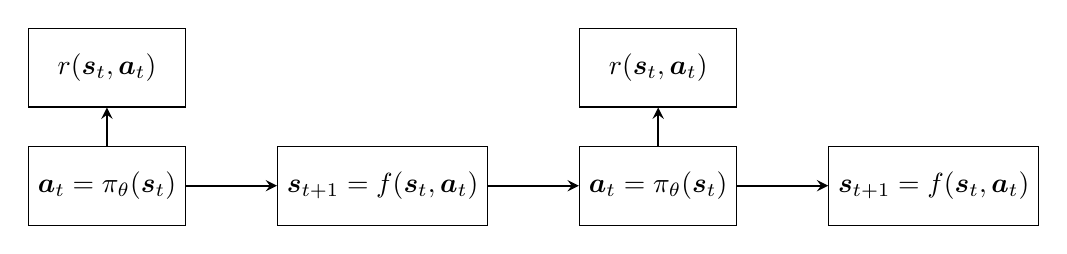
\begin{tikzpicture}[scale=1, transform shape, node distance=1.5cm]
		\node (action1) [rec] {$\bm{a}_{t} = \pi_\theta(\bm{s}_{t})$};
		\node (reward1) [rec, above of=action1] {$r (\bm{s}_{t}, \bm{a}_{t} )$};
		\draw [arrow] (action1) -- (reward1);
		\node (next_state1) [rec, right of=action1, xshift=2cm] {$\bm{s}_{t+1} = f (\bm{s}_{t}, \bm{a}_{t} ) $};
		\draw [arrow] (action1) -- (next_state1);
		\node (action2) [rec, right of=next_state1, xshift=2cm] {$\bm{a}_{t} = \pi_\theta(\bm{s}_{t})$};
		\draw [arrow] (next_state1) -- (action2);
		\node (reward2) [rec, above of=action2] {$r (\bm{s}_{t}, \bm{a}_{t} )$};
		\draw [arrow] (action2) -- (reward2);
		\node (next_state2) [rec, right of=action2, xshift=2cm] {$\bm{s}_{t+1} = f (\bm{s}_{t}, \bm{a}_{t} ) $};
		\draw [arrow] (action2) -- (next_state2);
\end{tikzpicture}
\end{center}
\end{figure}



\end{document}
